% !TEX encoding = UTF-8 Unicode
\documentclass[a4paper]{article}

\usepackage[utf8]{inputenc}
\usepackage{erk}
\usepackage{amsmath}
\usepackage{times}
\usepackage{graphicx}
\usepackage{hyperref}
\usepackage[top=22.5mm, bottom=22.5mm, left=22.5mm, right=22.5mm]{geometry}

\usepackage[slovene,english]{babel}

% local definitions
\def\footnotemark{}%  to avoid footnote on cover page

\begin{document}
%make title
\title{Potek napake funkcije atan2 ob popačenju vhodnih signalov}

\author{Mitja Alič} % use ^1, ^2 for author(s) from different institutions

\affiliation{Fakulteta za elektrotehniko, Univerza v Ljubljani, Tržaška cesta 25, 1000 Ljubljana}

\email{E-pošta: mitja1357@gmail.com}

\maketitle


\begin{abstract}{The course of error due to distortion of input signal to the atan2 function}
Distortion of sine and cosine values, used for angle determination with the atan2 function, can result in numerical error. According to the performed review of literature, error is normally presented by taking only the basic harmonic into account. This paper however presents determination of error by taking into account also higher harmonics, which are non-negligible at larger distortion of sine or cosine. Error is going to be expressed with infinite series, which expand the domain of distortion parameter. 
\end{abstract}


\selectlanguage{slovene}

\section{Uvod}

Dandanes je potreba po kakovostni regulaciji elektromotorskih pogonov neizogibna in tako prisotna v številnih aplikacijah. Za kakovostno nadzorovanje rotirajočega pogona, se v povratnih zankah uporablja senzorje zasuka \cite{uporaba_senzorjev}. Zasuk se meri na različne principe, inkrementalni dajalnik, resolver, enkoder \cite{inkrementalni}\cite{resolver}\cite{enkoder}... Izhoda enkoderja ali resolverja, sta signala sinus in kosinus. Za izračun informacije o zasuku se uporabi funkcijo inverz tangensa \cite{mat1}. V aplikacijah se običajno uporablja funkcija atan2, katere zaloga vrednosti je $[-\pi, \pi]$ \cite{atan}. 


Senzorji niso idealni in posledično je iluzorno pričakovati delovanje povsem brez napake. Primer napake je popačena oblika, zajetih signalov sinus in kosinus. Različne literature \cite{RLS1}, \cite{RLS2}, \cite{RLS3} opisujejo, kako popačenje vhodnih signalov vpliva na napako. Napako so izrazili le z najočitnejšimi harmoniki. V napaki nastopajo tudi višji harmoniki, katere se lahko predstavi kot napako v obliki neskončne vrste. V raznih aplikacijah je možen dostop le do izhodnega podatka o zasuku. Z referenčnim dajalnikom, se lahko določi napako, njen izvor ostaja neznan.

S poznavanjem vplivov popačenja signalov sinus in kosinus na napako, se lahko kasneje iz napake oceni kaj nanjo vpliva in kako jo zmanjšati.
V tem delu, bom predstavil, kako se pri popačenih vhodnih signalih sinusa in kosinusa  izraža napaka izračunanega kota v obliki neskončne vrste.


\section{Metodologija in rezultati}

Osnovna vhodna signala v funkcijo sta sinus in kosinus. Popačena sta lahko na več načinov:
\begin{eqnarray}
\label{equ:def_sin}
&Sin = B_{0} + B_1 \sin(\theta + \varphi_{s})\\
\label{equ:def_cos}
&Cos = A_{0} + A_1 \cos(\theta + \varphi_{c})
\end{eqnarray}
Vsebujeta lahko različne amplitude, fazne zamike ali enosmerne komponente. Idealno so v (\ref{equ:def_sin}) in (\ref{equ:def_cos}), $B_0$, $A_0$, $\varphi_{s}$ in $\varphi_{c}$, enaki 0, $B_1$ in $A_1$ sta enaka. Signaloma se lahko zaradi enega parametra spremeni tako amplituda kot faza. To se zgodi ob upoštevanju enega od parametrov v (\ref{equ:def_eks_sin}) in (\ref{equ:def_eks_cos}).
\begin{eqnarray}
\label{equ:def_eks_sin}
&Sin = \sin(\theta)+\Delta_c \cos(\theta)+\Delta_s \sin(\theta)\\
\label{equ:def_eks_cos}
&Cos =\cos(\theta)+\Delta_c \cos(\theta)+\Delta_s \sin(\theta)
\end{eqnarray}

Definicija merjenega kota $\varphi$ in  napake $\varepsilon$ je:

\begin{eqnarray}
\label{equ:def_kot}
&\varphi = \mathrm{atan2d}(Sin,Cos)\\
\label{equ:def_err}
&\varepsilon =\varphi - \mathrm{atan2d}(\sin(\theta),\cos(\theta))
\end{eqnarray}
pri čemer $\theta$ predstavlja referenco. atan2d() je funkcija, ki je že privzeto definirana v programskem okolju MATLAB in je namenjena izračunu vrednosti arkus tangensa v štirih kvadrantih. Izhod funkcije je podan v kotnih stopinjah \cite{atand}.
Napaka bo predstavljena v obliki neskončne vrste (\ref{equ:potek_napake}).
\begin{equation}
\label{equ:potek_napake}
\varepsilon(x) = C_0(x) + \sum_{n=1}^{\infty} C_n(x) \sin(n \Theta+ \varphi_n(x))
\end{equation}
Parameter x predstavlja, neodvisno spremenljivko, katera popači vhodna signala sinus in kosinus. $C_0$ predstavlja enosmerno komponento napake, $C_n$ amplitudo posameznega člena vrste ter $\varphi_n$ fazni zamik harmonika napake. Vsi členi so odvisni od x.



V nadaljevanju je predstavljen eden od možnih načinov določanja napake. Izbran parameter ($A_0$, $B_0$, $A_1$, $B_1$, $\varphi_{s}$, $\varphi_{c}$, $\Delta_s$, $\Delta_c$), katerega sem upošteval pri napaki, sem limitiral v neskončnost. Pri limitiranju parametra v neskončnost, se napaka izrazi v obliki npr:
\begin{equation}
\label{equ:def_err_inf}
\varepsilon=
\begin{cases}
90^\circ-\theta, & \theta \in \{0^\circ,180^\circ\}\\
270^\circ-\theta, & \theta \in \{180^\circ,360^\circ\}
\end{cases}
\end{equation}
Napako se da razviti v Fourierovo vrsto \cite{fourier} in s tem ugotoviti, konvergenco ter katere harmonike je potrebno opazovati. Sledi iskanje analitične funkcije, ki opisuje potek amplitude harmonika ter faznega zasuka posameznega harmonika, ob spremembi parametra. Raziskave so pokazale, da so višji harmoniki potence osnovnega harmonika napake. Napaka se izrazi kot potenčna vrsta.

V nadaljevanju so predstavljeni principi določanja napake, od različnih amplitudah, faznih zamikih, enosmernih komponentah, ter kombinaciji različnih amplitud ter faz zaradi parametra $\Delta_s$ ali $\Delta_s$.

\subsection{Določanje napake ob različnih amplitudah}

Definirajmo razmerje amplitude sinusa in kosinusa s $k$. Sprememba obeh amplitud za določen faktor ne bo ustvarila dodatne napake.
	\begin{eqnarray}
	\label{equ:def_sin_ama}
	&Sin = k \sin(\theta)\\
	\label{equ:def_cos_amp}
	&Cos =\cos(\theta)
	\end{eqnarray}
Ob povečanju $k$ proti neskončnosti, se pojavi napaka (slika \ref{fig:lim_amp}),
\begin{equation}
\label{equ:amp_lim}
\lim_{k \rightarrow \infty} (\mathrm{atan2}(k \sin{\theta},\cos{\theta})-\mathrm{atan2}(\sin{\theta},\cos{\theta}))
\end{equation}
\begin{figure}[!htb]
	\begin{center}
		\includegraphics[width=\linewidth]{./Slike/lim_amp.eps}
		\caption{Napaka $\varepsilon$ ob limiti $k$ proti neskončnosti} \label{fig:lim_amp}
	\end{center}
\end{figure}

ki se v Fourierovi vrsti izrazi kot:
\begin{equation}
\label{equ:lim_amp_vrsta}
\varepsilon = \frac{180}{\pi}\sum_{n=1}^{\infty}\frac{1}{n} \sin 2 n \theta.
\end{equation}
Največji vpliv ima drugi harmonik, njegov potek v odvisnoti od $k$ je predstavljen na sliki \ref{fig:amp} kot $C_1$, saj nastopajo le sodi harmoniki.
\begin{figure}[!htb]
	\begin{center}
		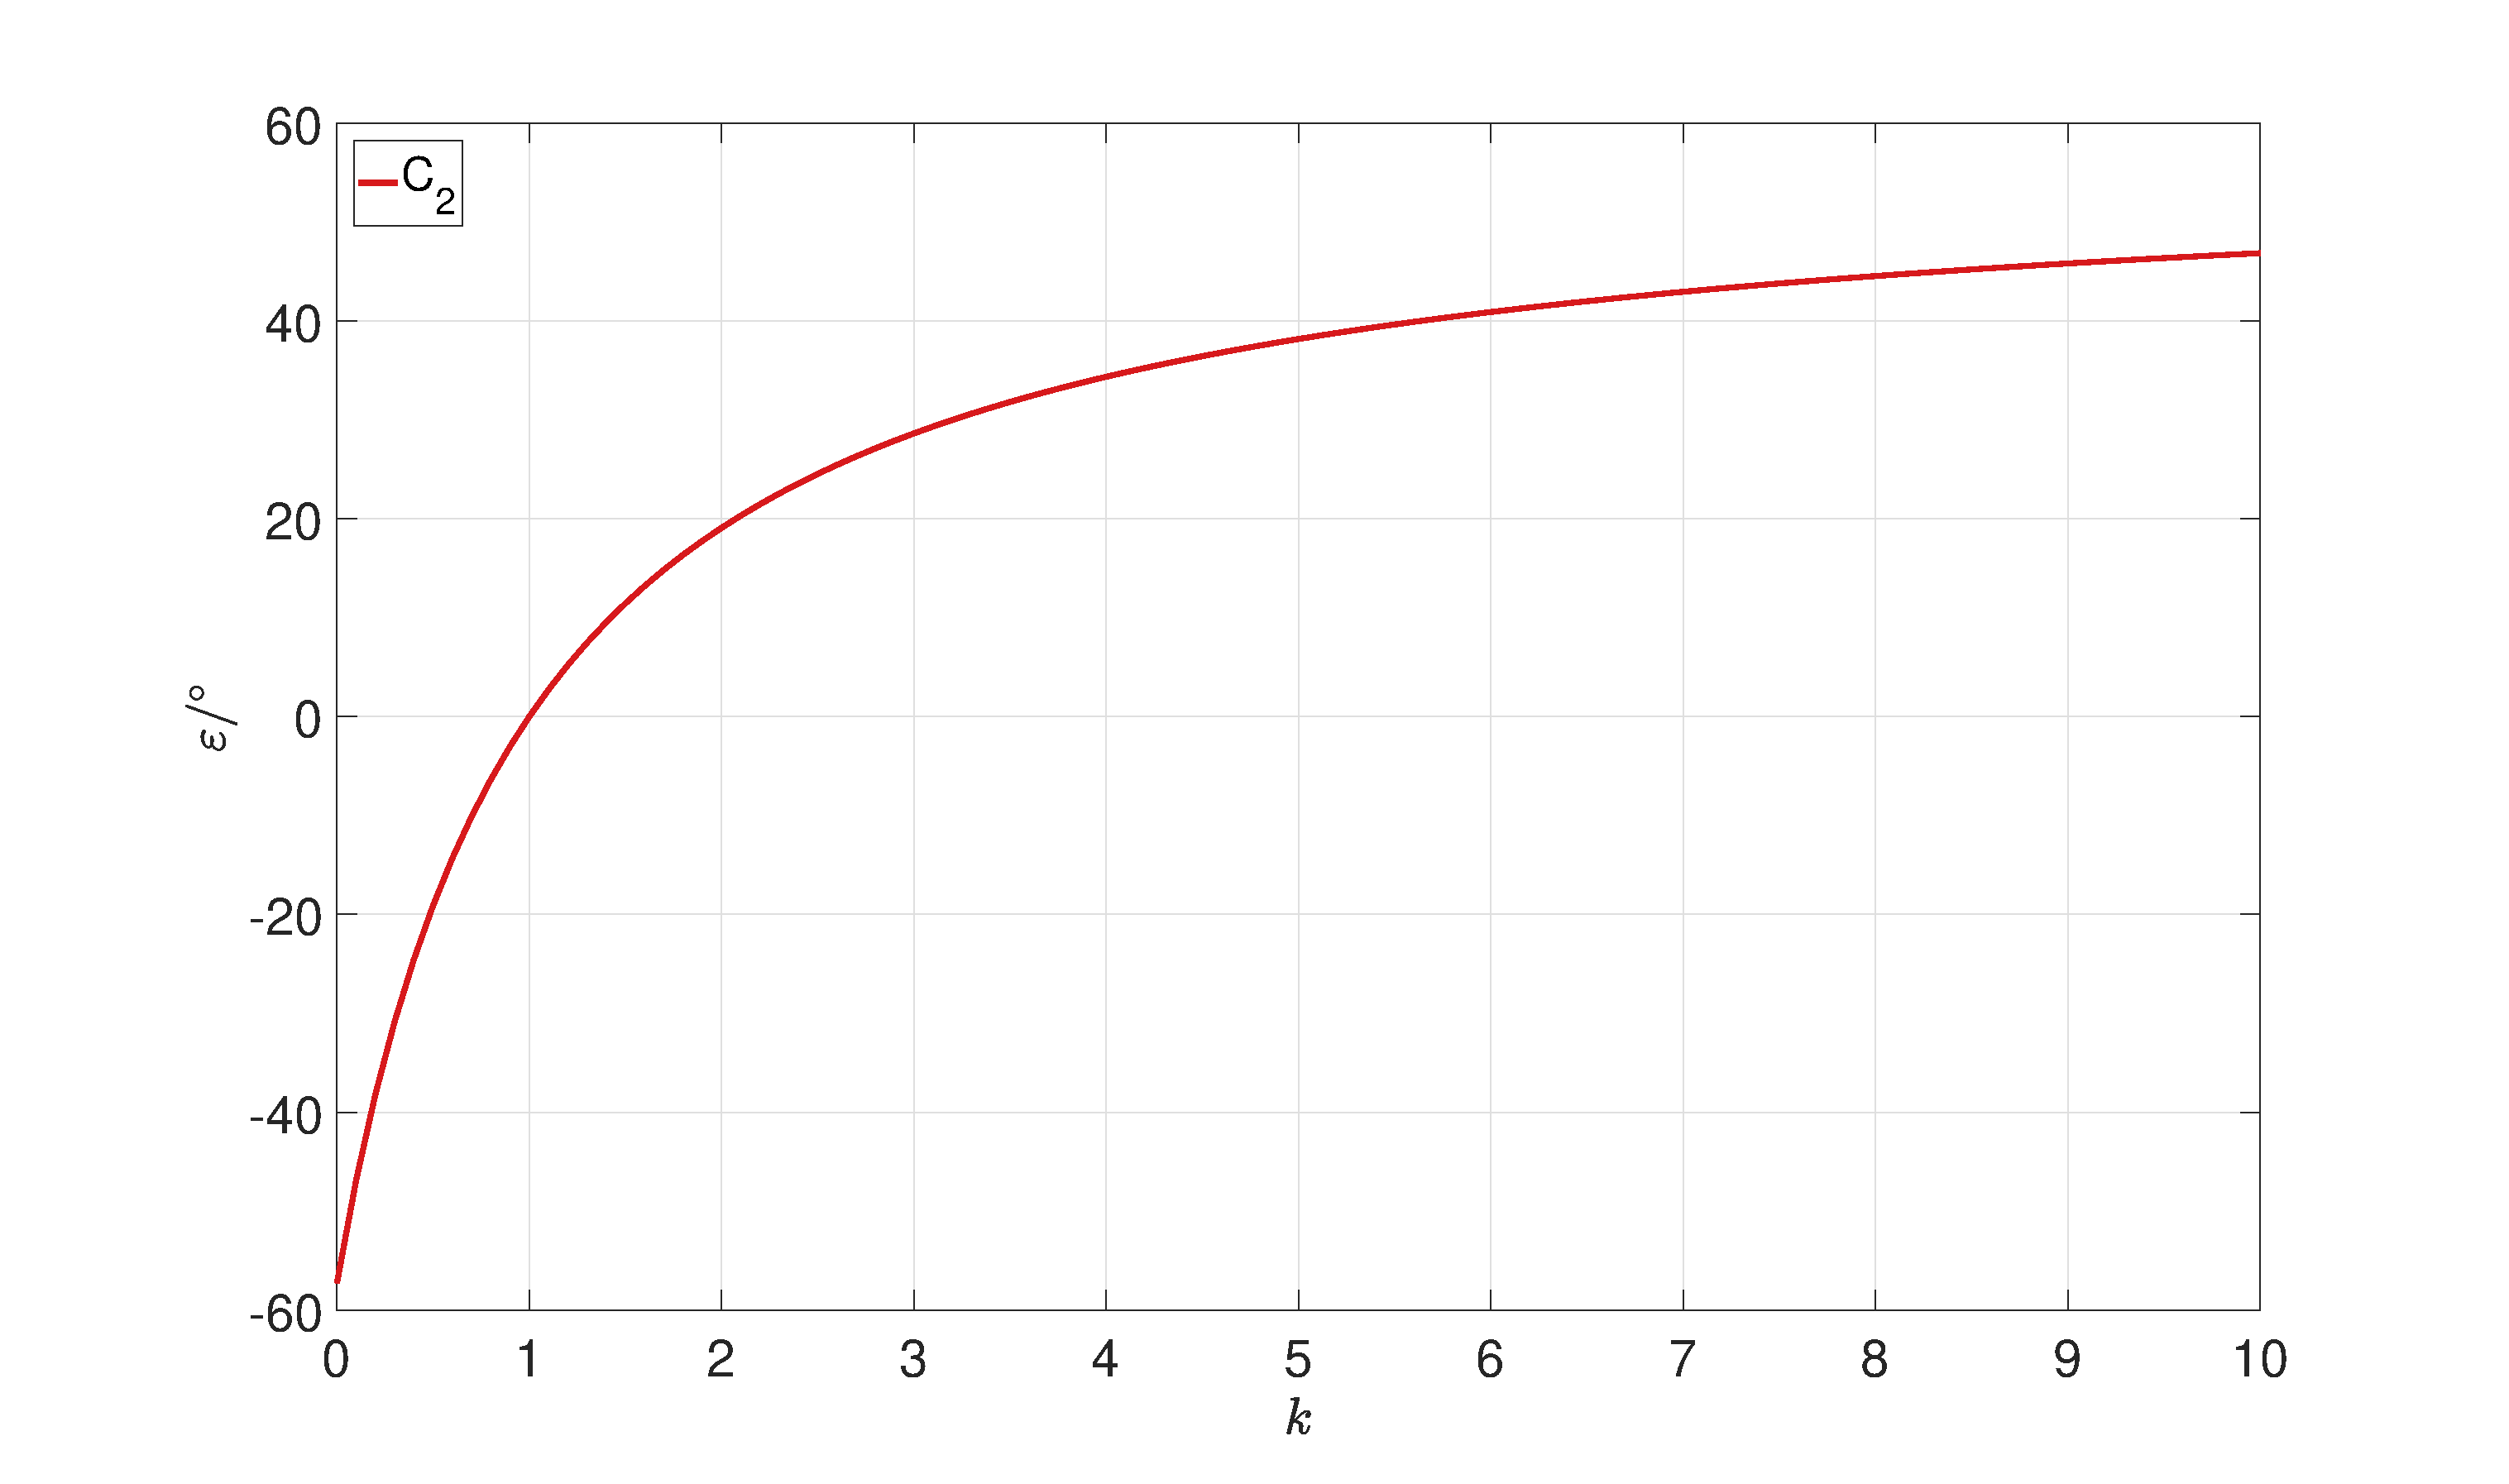
\includegraphics[width=\linewidth]{./Slike/amp.eps}
		\caption{Potek drugega harmonika v odvistnosti od $k$} \label{fig:amp}
	\end{center}
\end{figure}

Z uporabo Curve Fitting Toolbox se poteku, najbolje prilega  racionalna funkcija. Napaka se izrazi s potenčno vrsto:

\begin{equation}
\label{equ:amp_err}
\varepsilon(k) =\frac{180}{\pi}\sum_{n=1}^{\infty}\frac{1}{n}(\frac{k-1}{k+1})^n \sin 2 n \theta
\end{equation}

in velja, če je $k$ večji od 0.$$k \geq 0$$

V (\ref{equ:amp_err}) namesto $k$ vstavimo razmerje amplitud:
\begin{equation}
\label{equ:amp_err2}
\varepsilon(k) =\frac{180}{\pi}\sum_{n=1}^{\infty}\frac{1}{n}(\frac{B_1-A_1}{B_1+A_1})^n \sin 2 n \theta
\end{equation}
kar velja pri pogoju: $$\frac{B_1}{A_1} \geq 0.$$

\subsection{Določanje napake ob spremembi faznega zamika}


Vhodna signala imata naslednjo obliko:
\begin{eqnarray}
\label{equ:def_sin_fis}
&Sin = \sin(\theta + \varphi_{s})\\
\label{equ:def_cos_fis}
&Cos =\cos(\theta+\varphi_{c})
\end{eqnarray}
Napako se določi posamično za vsakega od parametrov. Drugi je takrat enak 0. Na koncu se enačbi združi. Za določanje limite ni potrebno iti proti neskončnosti, ampak le do najslabše možnosti, ki je pri $\pm 90^\circ$:
\begin{equation}
\label{equ:fis_lim}
\varepsilon = \lim_{\varphi_{s} \rightarrow 90^\circ} \mathrm{atan2}(Sin ,Cos)- \mathrm{atan2d}(\sin(\theta),\cos(\theta))
\end{equation}
Potek napake $\varepsilon$ s slike \ref{fig:lim_sin_fis} predstavi vrsta (\ref{equ:lim_fis_vrsta}).
\begin{figure}[!htb]
    \begin{center}
        \includegraphics[width=\linewidth]{./Slike/lim_sinfaza.eps}
        \caption{Napaka $\varepsilon$ ob limiti $\varphi_{s} \rightarrow 90^\circ$} \label{fig:lim_sin_fis}
    \end{center}
\end{figure}
\begin{equation}
\label{equ:lim_fis_vrsta}
\varepsilon = 45^\circ - \frac{180}{\pi}\sum_{n=1}^{\infty}\frac{1}{n} \sin (2n \theta)
\end{equation} 
Iz  izraza je vidno nastopanje enosmerne komponente in sodih harmonikov. Na sliki \ref{fig:fis} so prikazani: potek enosmerne komponente $C_0$, potek amplitude drugega harmonika $C_1$, in $\varphi_1$ fazni zamik drugega harmonika glede na kosinusno obliko. Za predstavitev poteka s sinusi, je potrebno prišteti še $90^\circ$. Ordinatna skala grafa na sliki \ref{fig:fis} je v stopinjah. Pri $C_0$ in $C_1$, stopinje predstavljajo amplitudo napake, pri $\varphi_{1}$ skala prikazuje fazni zamik v stopinjah.
\begin{figure}[!htb]
	\begin{center}
		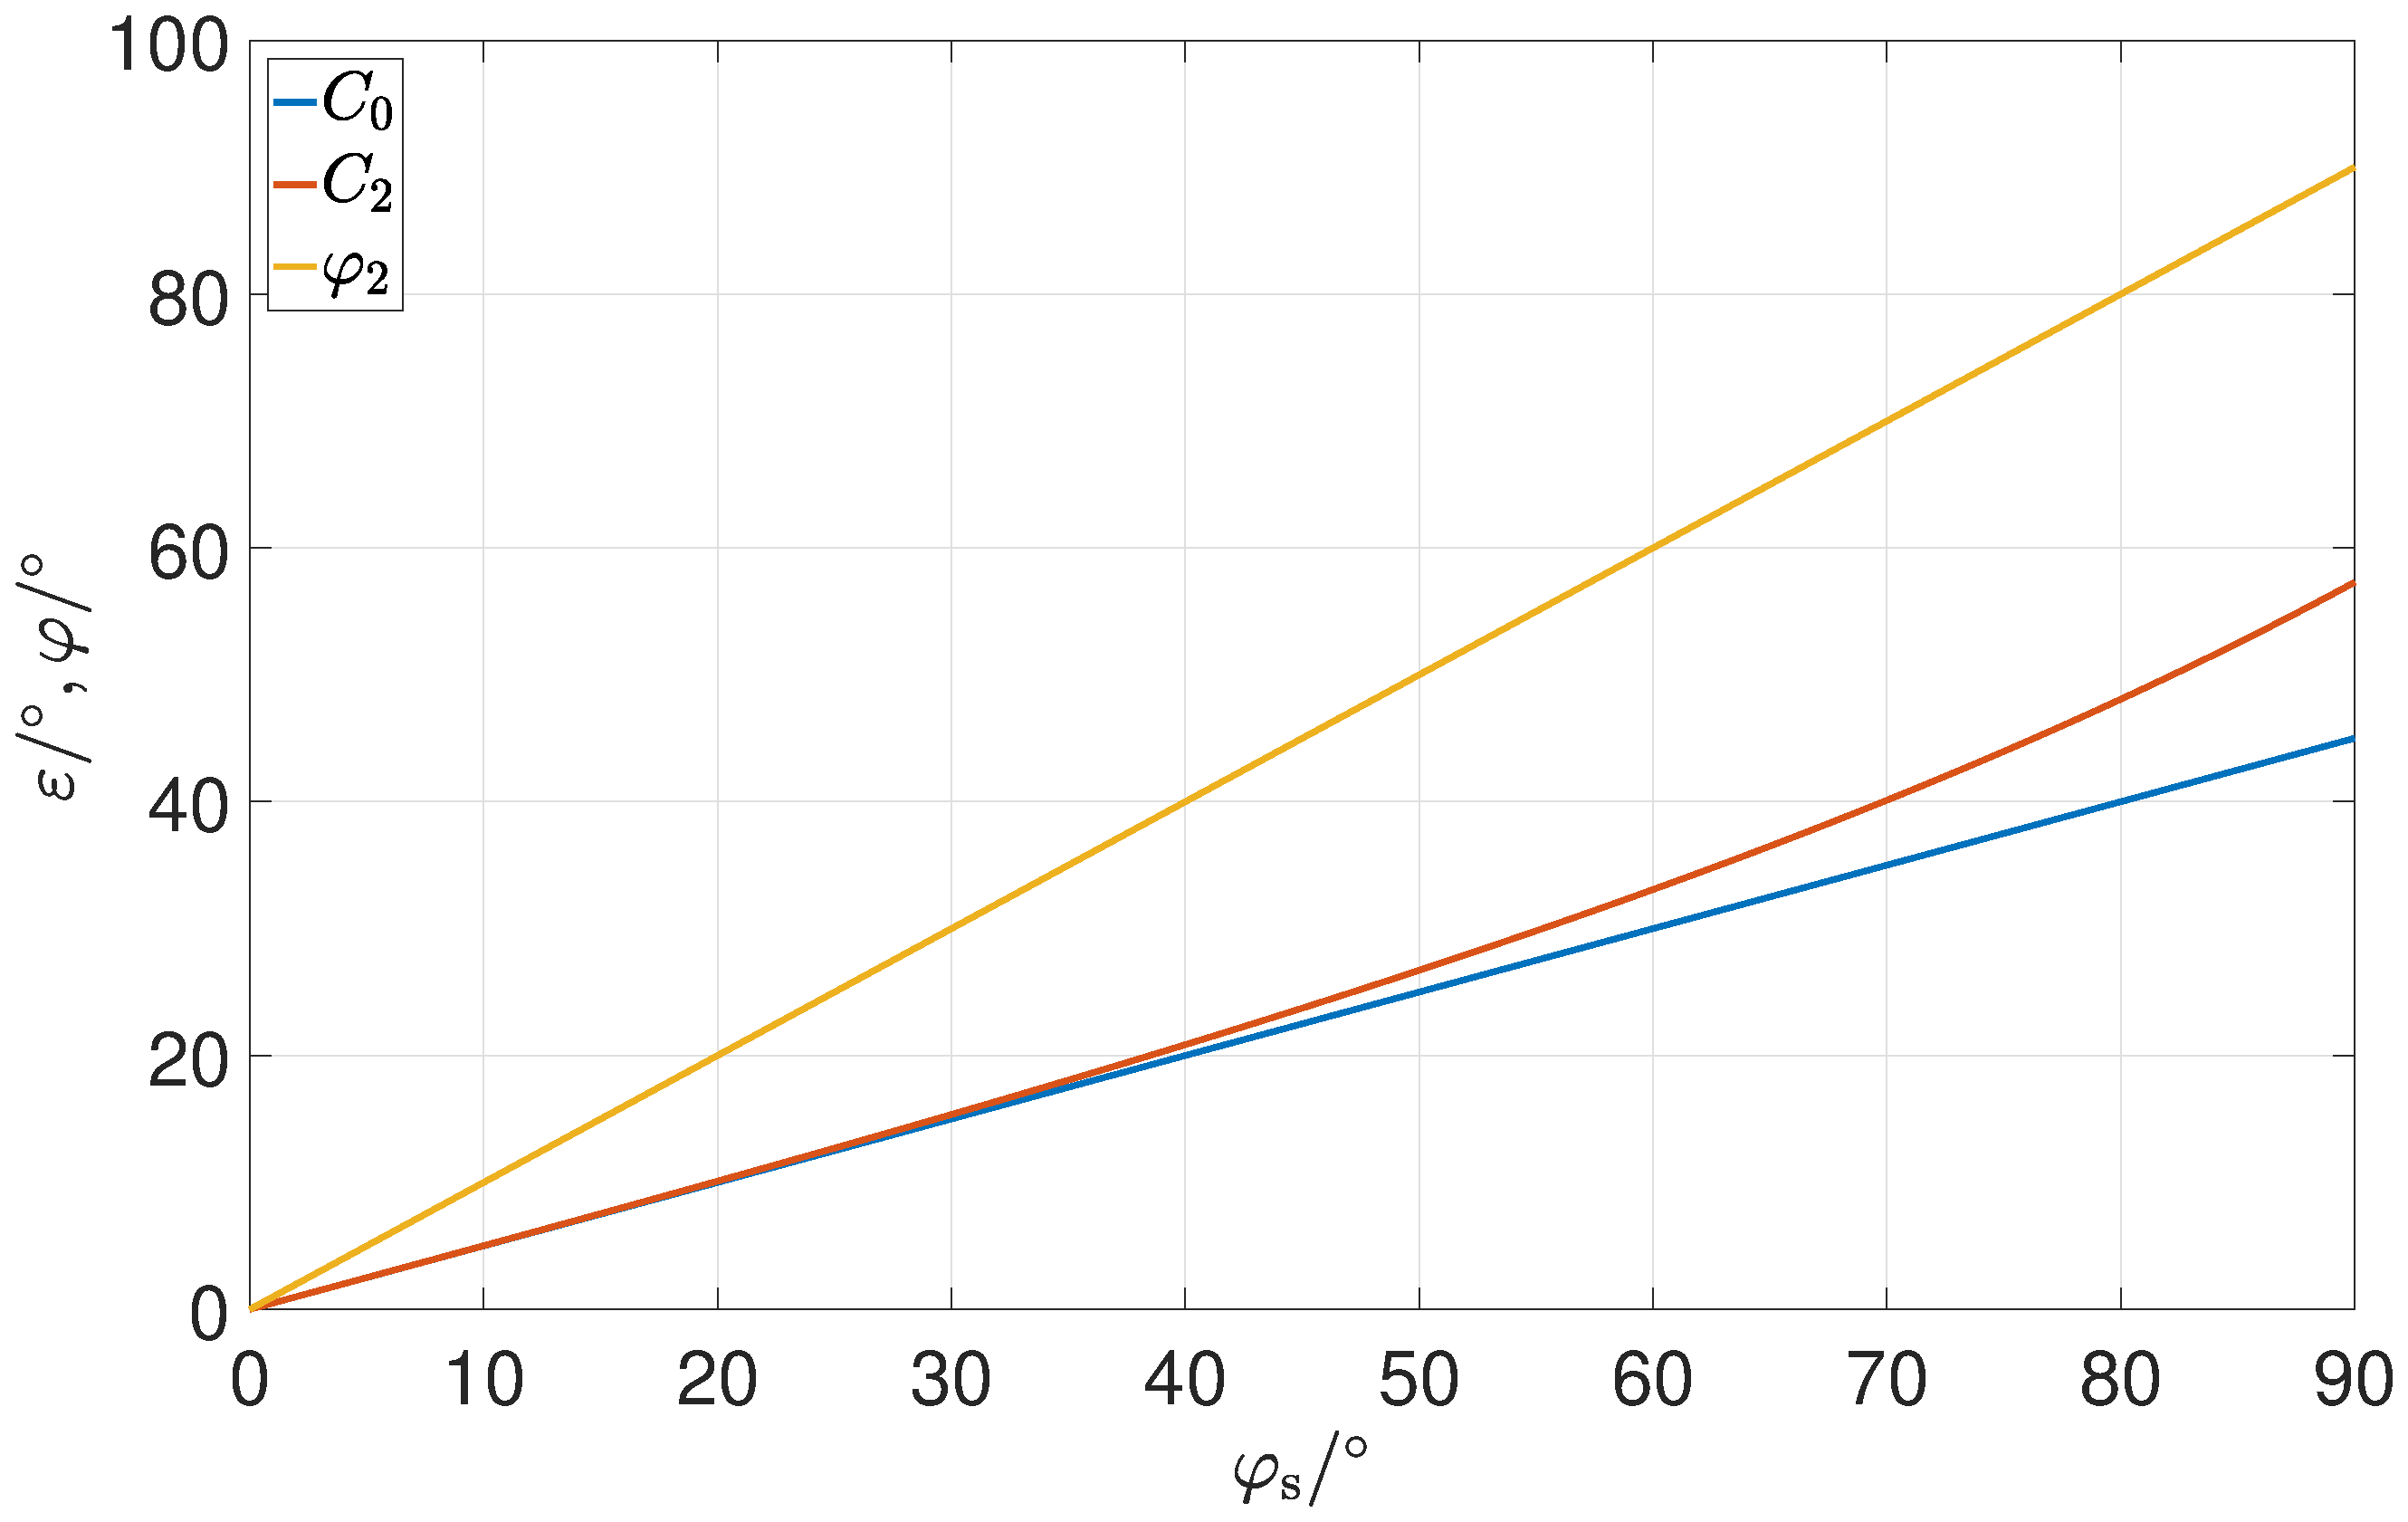
\includegraphics[width=\linewidth]{./Slike/fis.eps}
		\caption{Potek enosmerne komponente napake $C_0$, amplitude drugega harmonika $C_1$ in faznega zamika $\varphi_1$ glede na kosinus, v odvistnisti od faznega zamika sinusa $\varphi_{s}$} \label{fig:fis}
	\end{center}
\end{figure}
Poteku enosmerne komponte se najbolje prilega funkcija premice.
Potek amplitude drugega harmonika napake ima obliko funkcije tangens.
Fazni zamik drugega harmonika narašča linearno, vendar je za predstavitev s sinusi potrebno prišteti še $90^\circ$. Enako se lahko ponovi za fazni zamik kosinus signala.
Enačba končnega poteka se glasi:
\begin{multline}
\label{equ:fis_err}
\varepsilon(\varphi_{s},\varphi_{c}) = \frac{\varphi_{s}+\varphi_{c}}{2}+\\ \frac{180}{\pi}\sum_{n=1}^{\infty}\frac{1}{n} (\mathrm{tan}\frac{\varphi_{s}-\varphi_{c}}{2})^n \sin (2n \theta+n(90^\circ +\varphi_{s}+\varphi_{c}))
\end{multline}
pri čemer, enačba velja za :
$$ \varphi_{s}-\varphi_{c} \in [ -90^\circ , 90^\circ ] $$

\subsection{Določanje napake ob spremembi enosmerne komponente}
Amplitudi sigalov sinus in kosinus sta enaki 1.
Z limito $A_0$ in razvojem napake v Fourierovo vrsto napako izrazimo z:
\begin{equation}
\label{equ:off_lim_vrsta}
\varepsilon = \frac{180}{\pi}\sum_{n=1}^{\infty}\frac{2}{n} \sin (n \theta+ 90^\circ n).
\end{equation}
Enosmerne komponente ni,  največji je prvi harmonik.
\begin{figure}[!htb]
	\begin{center}
		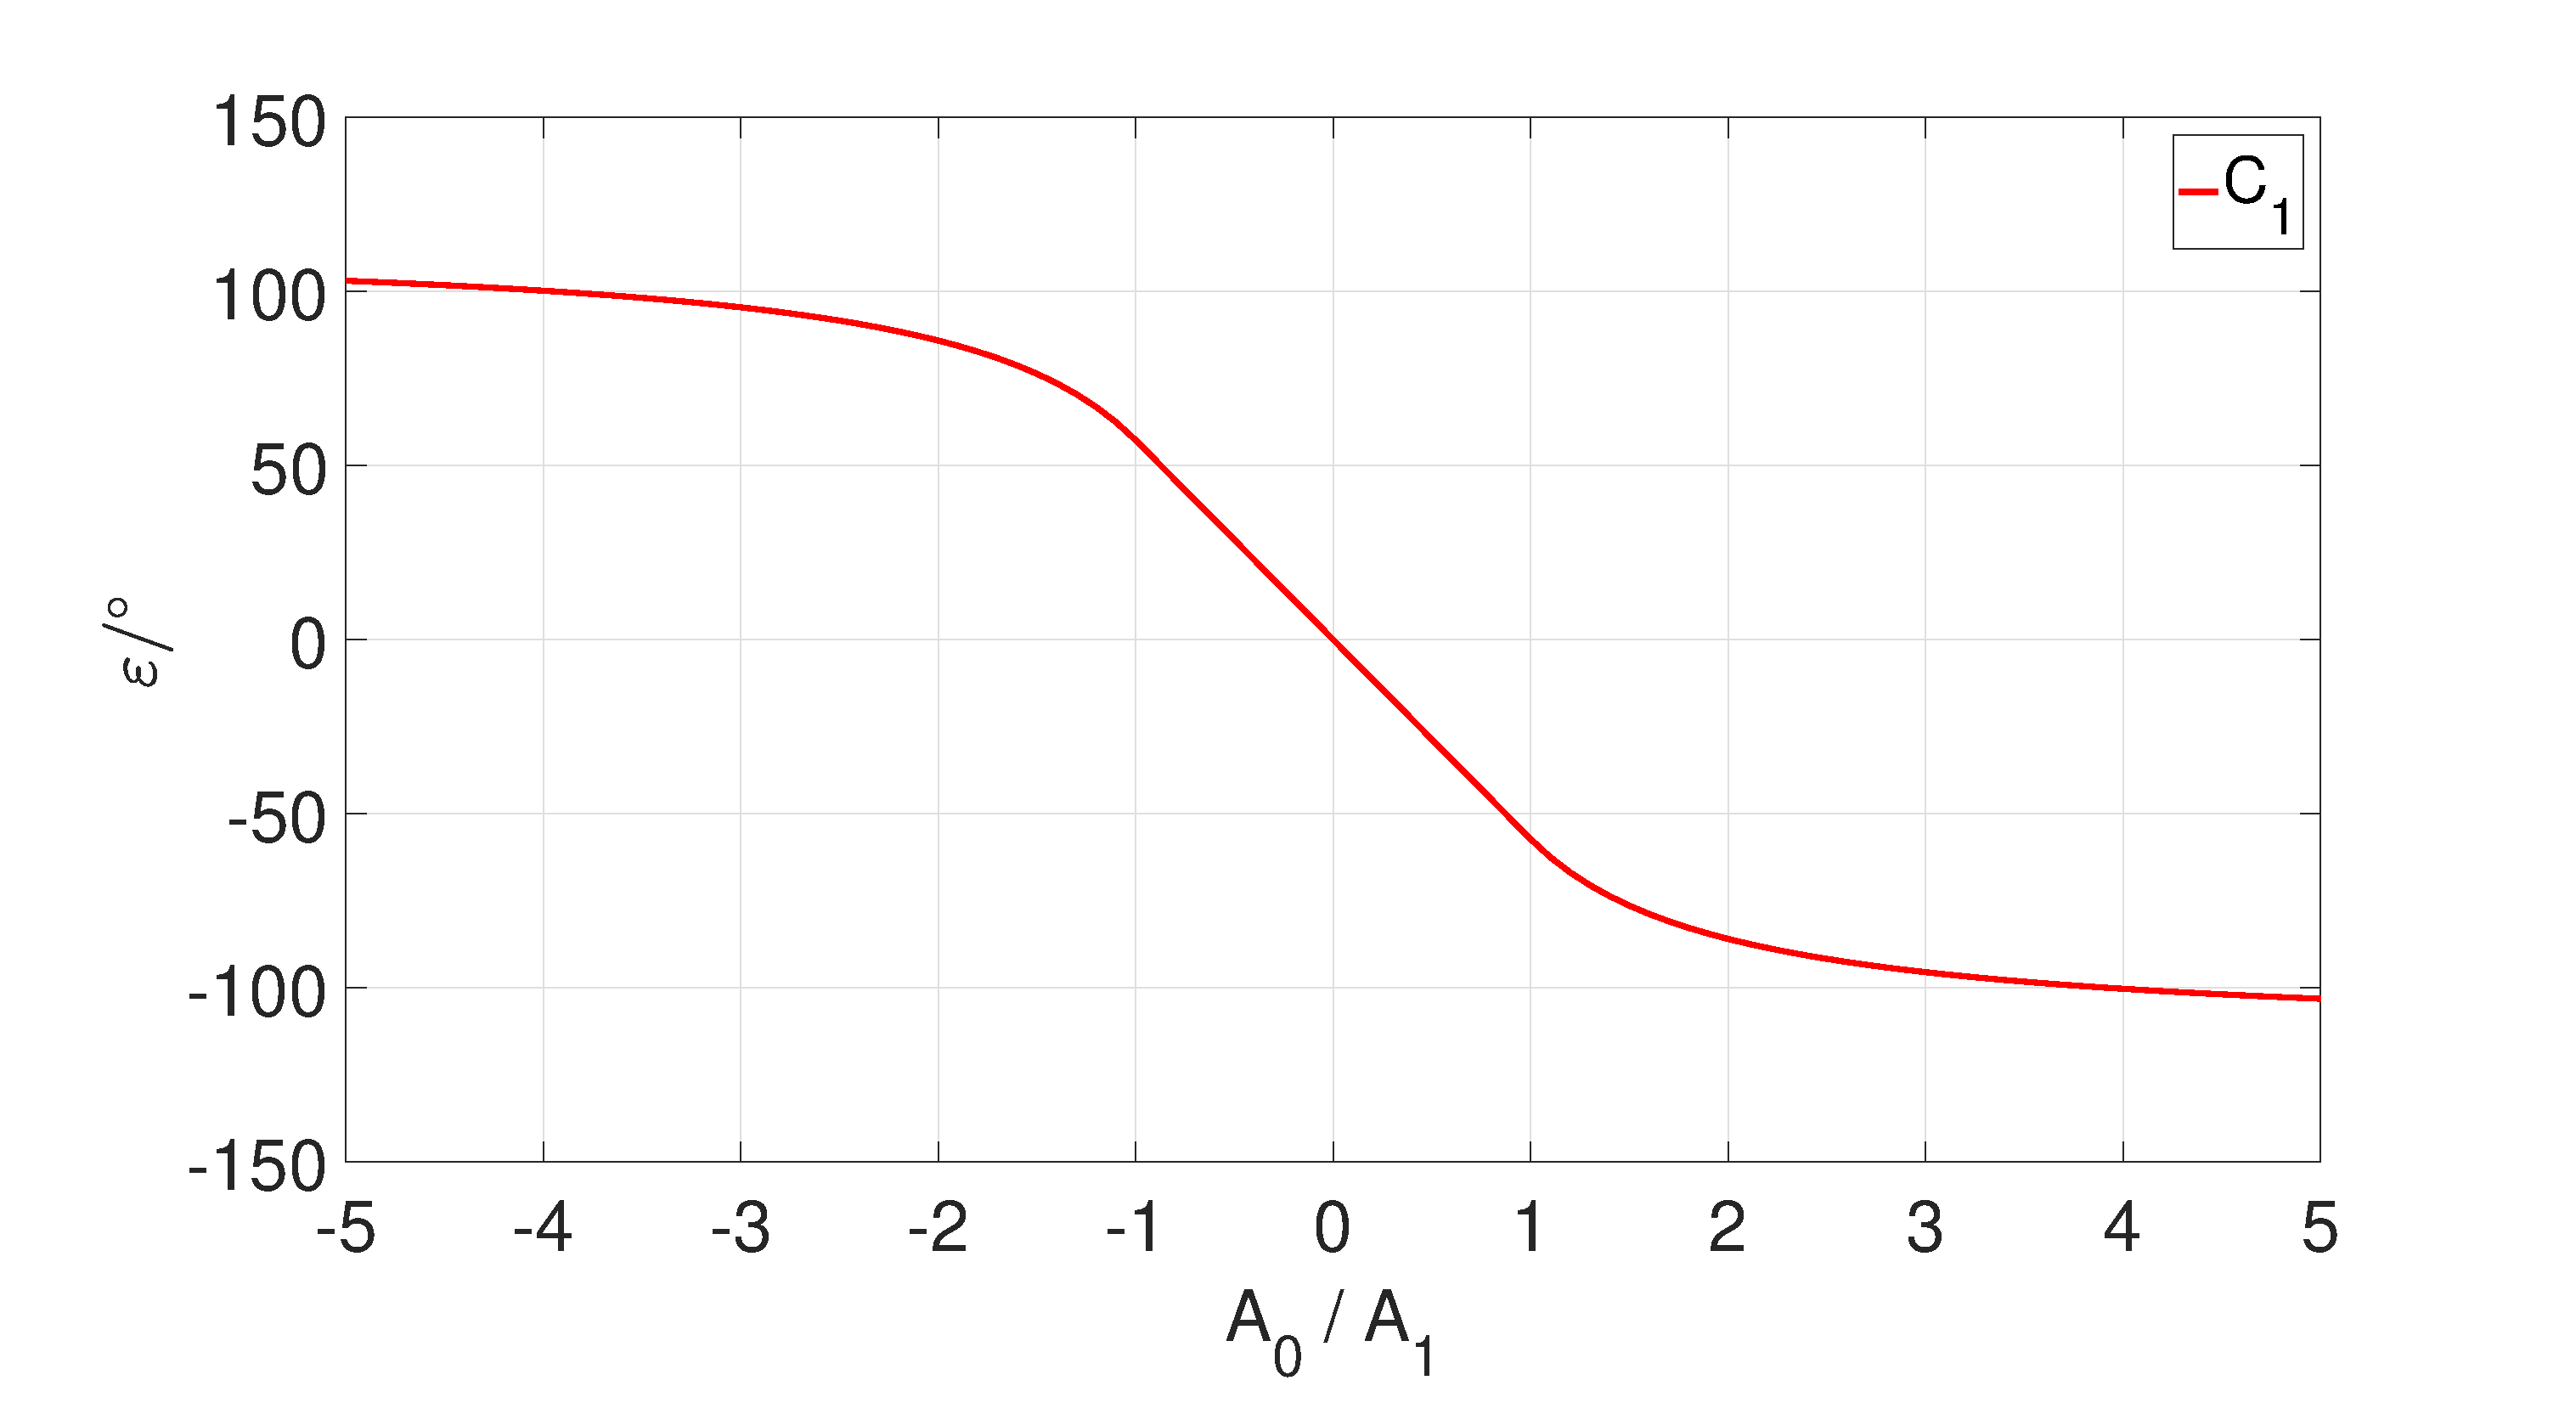
\includegraphics[width=\linewidth]{./Slike/off.eps}
		\caption{Potek amplitude prvega harmonika od enosmerne komponente kosinus signala, pri amplitudah enakih 1} \label{fig:off}
	\end{center}
\end{figure}
Potek s slike \ref{fig:off} se razdeli na 3 dele in aproksimira napako z naslednjim izrazom upoštevajoč tudi enakosti amplitud:
\begin{multline}
\label{equ:offc_err}
\varepsilon(A_0)=\\
\begin{cases}
\frac{180}{\pi}\sum_{n=1}^{\infty}(-1)^n\frac{1}{n}(2-|\frac{A_0}{A_1}|^{-n}) \sin (n \theta ), & \frac{A_0}{A_1}\leq -1 \\
\frac{180}{\pi}\sum_{n=1}^{\infty}(-1)^n\frac{1}{n}(\frac{A_0}{A_1})^n \sin (n \theta ), & |\frac{A_0}{A_1}|\leq 1 \\
\frac{180}{\pi}\sum_{n=1}^{\infty}(-1)^n\frac{1}{n}(2-(\frac{A_0}{A_1})^{-n}) \sin (n \theta ), & \frac{A_0}{A_1}\geq 1
\end{cases}
\end{multline}

Enako se lahko stori tudi za $B_0$ (\ref{equ:offs_err}) in za aproksimacijo napake, ko imata sinus in kosinus enako enosmerno komponento (\ref{equ:offsc_err}).

\begin{multline}
\label{equ:offs_err}
\varepsilon(B_0)=\\
\begin{cases}
\frac{180}{\pi}\sum_{n=1}^{\infty}\frac{1}{n}(2-|\frac{B_0}{B_1}|^{-n}) \sin (n \theta -  90^\circ n), & \frac{B_0}{B_1}\leq -1 \\
\frac{180}{\pi}\sum_{n=1}^{\infty}\frac{1}{n}(\frac{B_0}{B_1})^n \sin (n \theta + 90^\circ n), & |\frac{B_0}{B_1}|\leq 1 \\
\frac{180}{\pi}\sum_{n=1}^{\infty}\frac{1}{n}(2-(\frac{B_0}{B_1})^{-n}) \sin (n \theta^\circ + 90 n), & \frac{B_0}{B_1}\geq 1
\end{cases}
\end{multline}

\begin{multline}
\label{equ:offsc_err}
\varepsilon(A_0,B_0=A_0)=\\
\begin{cases}
\frac{180}{\pi}\sum_{n=1}^{\infty}\frac{1}{n}(2-|\sqrt{2}\frac{A_0}{A_1}|^{-n}) \sin (n \theta + 90^\circ n), & \frac{A_0}{A_1}\leq -\frac{\sqrt{2}}{2} \\
\frac{180}{\pi}\sum_{n=1}^{\infty}\frac{1}{n}(\sqrt{2}\frac{A_0}{A_1})^n \sin (n \theta - 90^\circ n), & |\frac{A_0}{A_1}|\leq \frac{\sqrt{2}}{2} \\
\frac{180}{\pi}\sum_{n=1}^{\infty}\frac{1}{n}(2-(\sqrt{2}\frac{A_0}{A_1})^{-n}) \sin (n \theta - 90^\circ n), & \frac{A_0}{A_1}\geq \frac{\sqrt{2}}{2}
\end{cases}
\end{multline}

\subsection{Različni amplitudi in fazi v odvistnosti od enega parametra}

Fourierova vrsta limite (\ref{equ:def_err}) pri upoštevanju (\ref{equ:def_eks_sin}) in (\ref{equ:def_eks_cos}), ko gre $\Delta_c$ v neskončnost je
\begin{equation}
\label{equ:lim_dc_vrsta}
\varepsilon = 45^\circ -\frac{180}{\pi}\sum_{n=1}^{\infty}\frac{1}{n} \sin( 2 n \theta).
\end{equation}

Potek drugega harmonika od $\Delta_c$ se lahko zapiše kot vsota sinusa in kosinusa.
\begin{equation}
C_{1s} \cdot\sin(2\theta)+C_{1c} \cdot\cos(2\theta)
\end{equation}
Poteki enosmerne komponente ter drugega harmonika predstavljenega kot seštevek sinusa in kosinusa so prikazani na sliki \ref{fig:dc}.
\begin{figure}[!htb]
	\begin{center}
		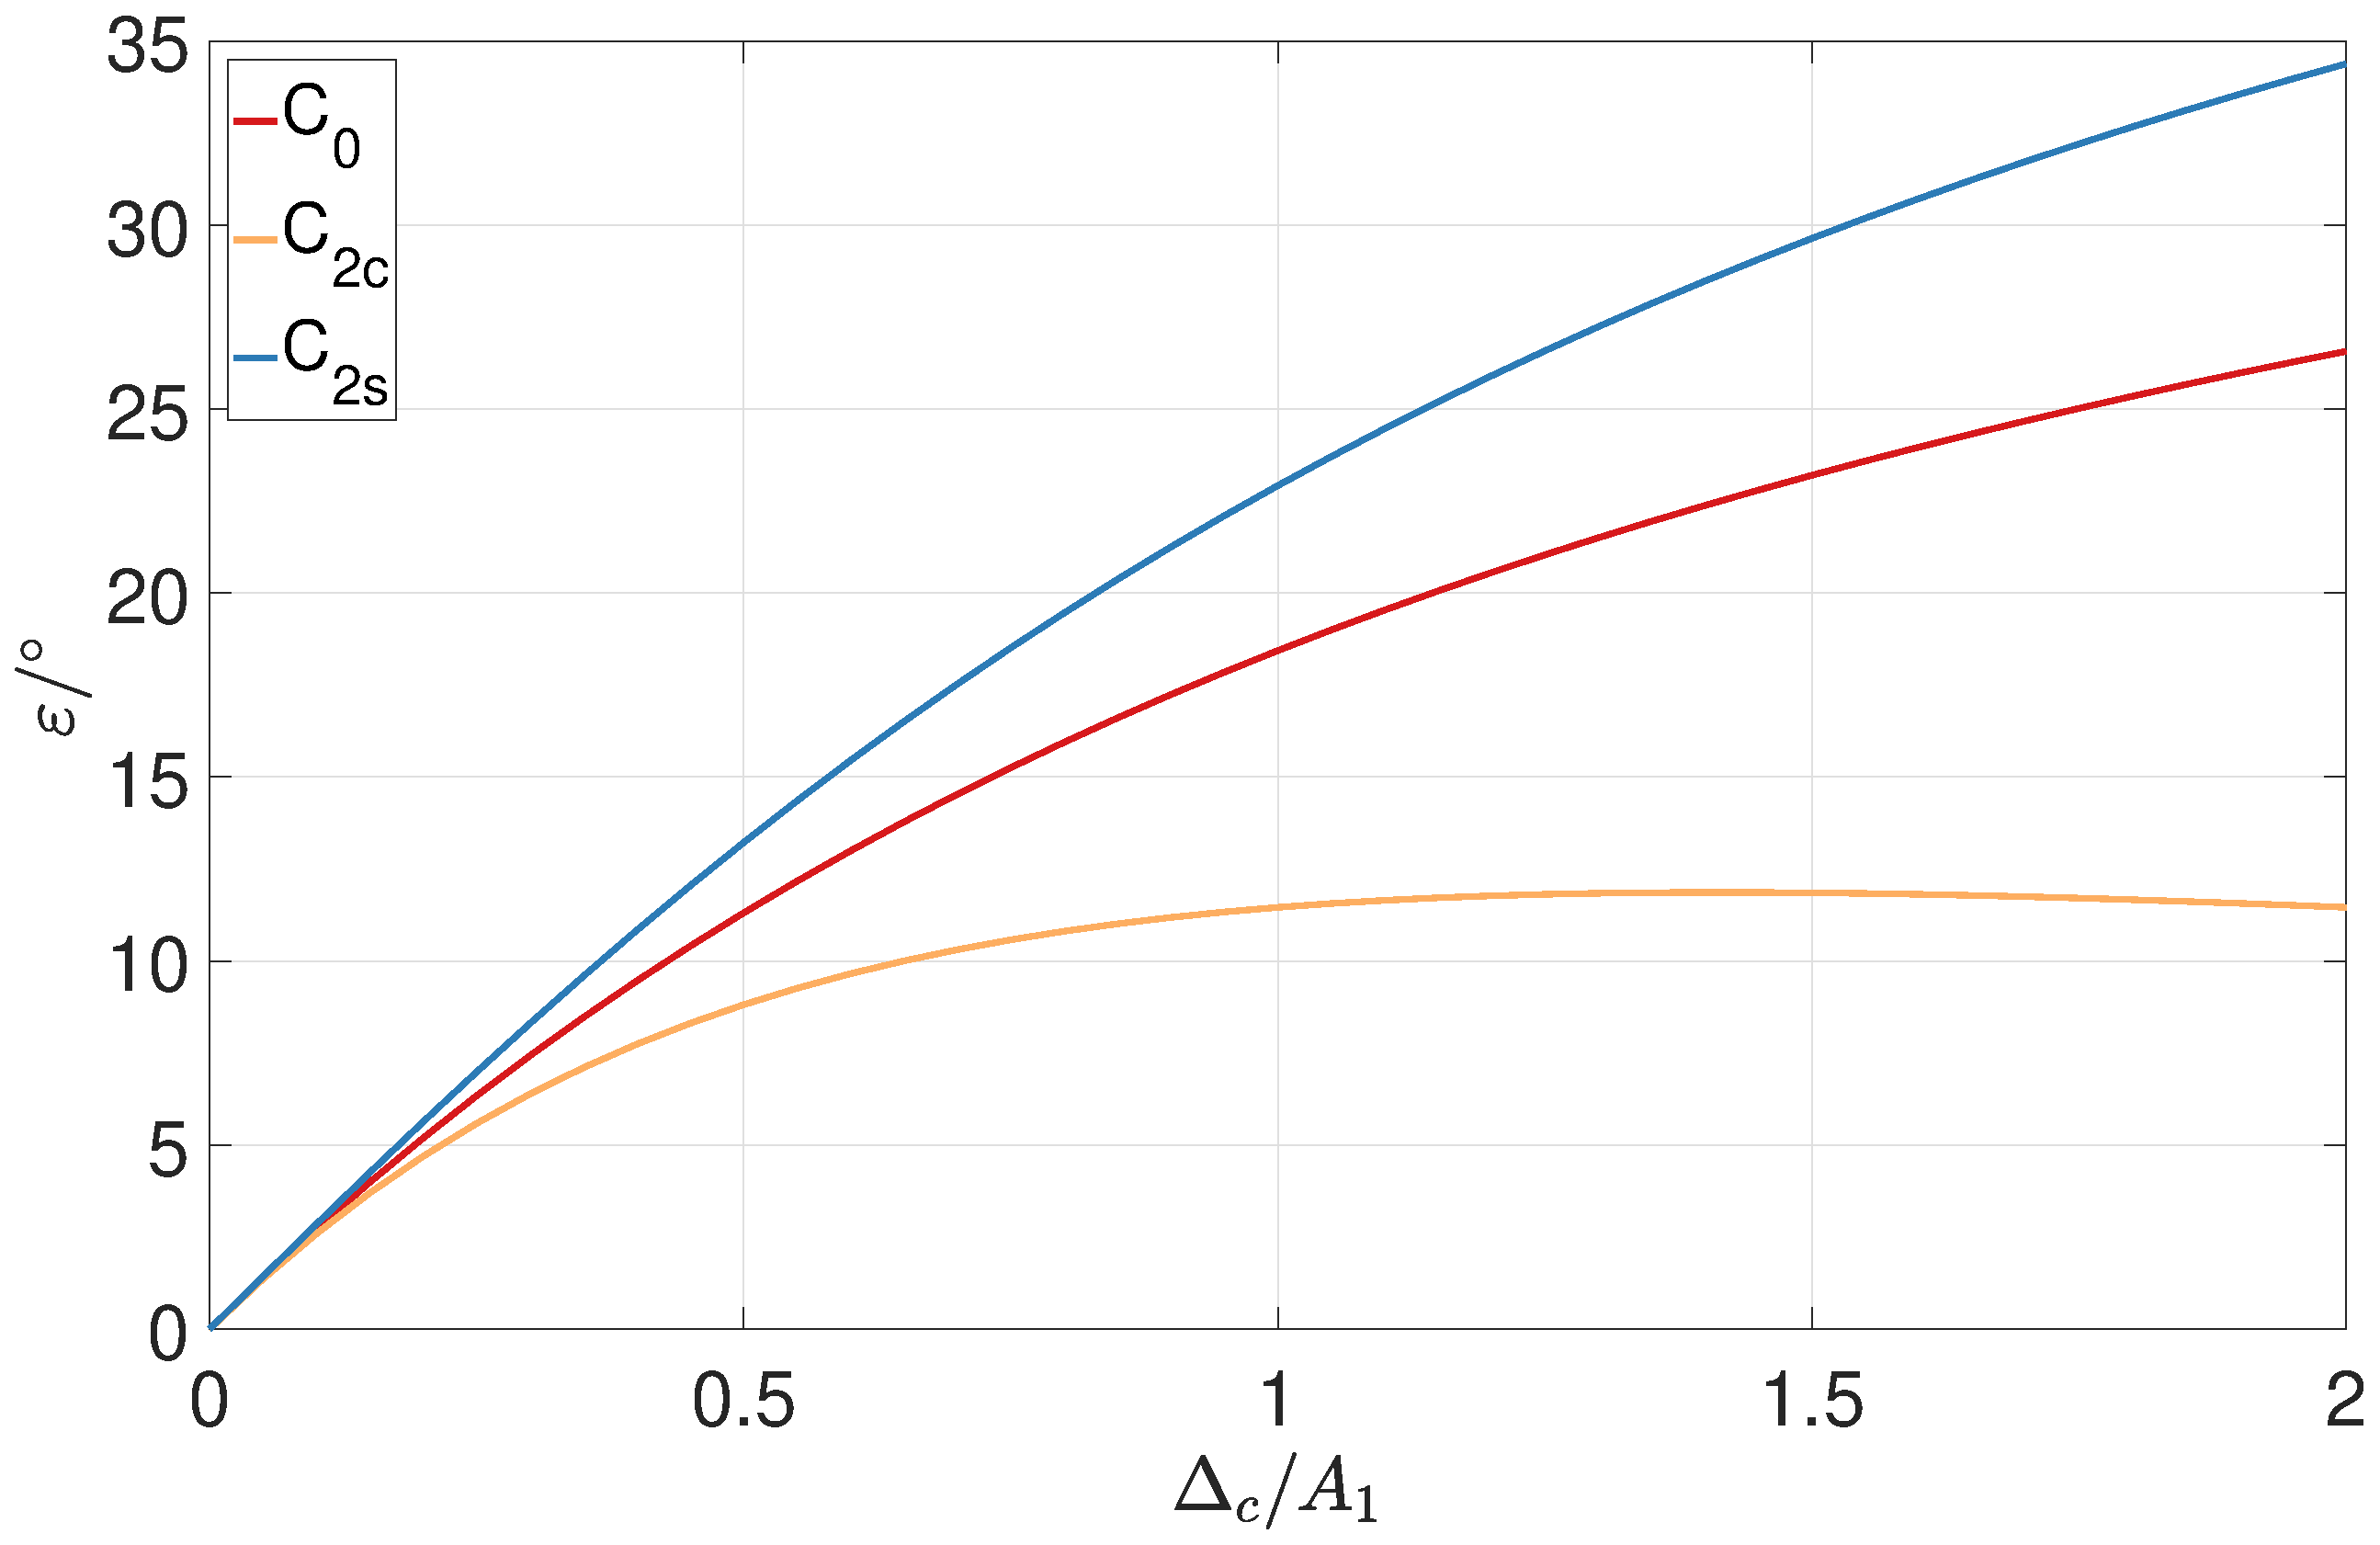
\includegraphics[width=\linewidth]{./Slike/dc.eps}
		\caption{Potek enosmerne komponente in drugega harmonika napake, v odvistnisti od $\Delta_{c}$} \label{fig:dc}
	\end{center}
\end{figure}

Enosmerna komponenta ima obliko racionalne funkcije v funkciji atan.
$C_1s$ in $C_1c$ sti racionalni funkciji. Amplituda je geometrijska vsota členov $C_n = \sqrt{C_{ns}^2+C_{nc}^2}$, faza za sinusni potek napake je $\varphi_{n} = atan(\frac{C_{nc}}{C_{ns}})$. Končna enačba z upoštevanjem amplitude osnovnega signala sinus in kosinus se glasi:

\begin{multline}
\label{equ:dc_err}
\varepsilon(\Delta_c) =\\ \mathrm{atand}\frac{\Delta_c}{\Delta_c+2 A_1}+\frac{180}{\pi} \sum_{n=1}^{\infty}\frac{1}{n} (\frac{\Delta_c}{\sqrt{\Delta_c^2+2 A_1 \Delta_c+2 A_1}})^n\\ \sin (2n \theta+n (90^\circ+ \mathrm{ atan}(\frac{\Delta_c+A_1}{A_1})))
\end{multline}
\begin{multline}
\label{equ:ds_err}
\varepsilon(\Delta_s) =\\ \mathrm{atand}\frac{-\Delta_s}{\Delta_s+2 A_1}+\frac{180}{\pi} \sum_{n=1}^{\infty}\frac{1}{n} (\frac{\Delta_s}{\sqrt{\Delta_s^2+2 A_1 \Delta_s+2A_1}})^n\\ \sin (2n \theta+n (90^\circ+ \mathrm{ atan}(\frac{\Delta_s+A_1}{A_1})))
\end{multline}
\begin{equation*}
\Delta_s, \Delta_c > -A_1
\end{equation*}



\section{Komentar rezultatov}
Pri modeliranju potekov, je bilo uporabljeno prvih 15 členov potenčne vrste. Razlika med dejansko napako in predvideno napako je le numerična (slika \ref{fig:razlika}). Opravil sem fft predvidene in dejanske napake. Razlika med posameznima amplitudama harmonika je le numerična. V primeru, da parameter dosega večje vrednosti, ali se približuje robnim pogojem, dejanska napaka postane nezvezna in je s 15 členi ni mogoče povsem določiti. Omenti je potrebno, da so kljub izpeljavam predstavljene vrste napake posameznih deformacij med seboj odvisne.
\begin{figure}[!htb]
	\begin{center}
		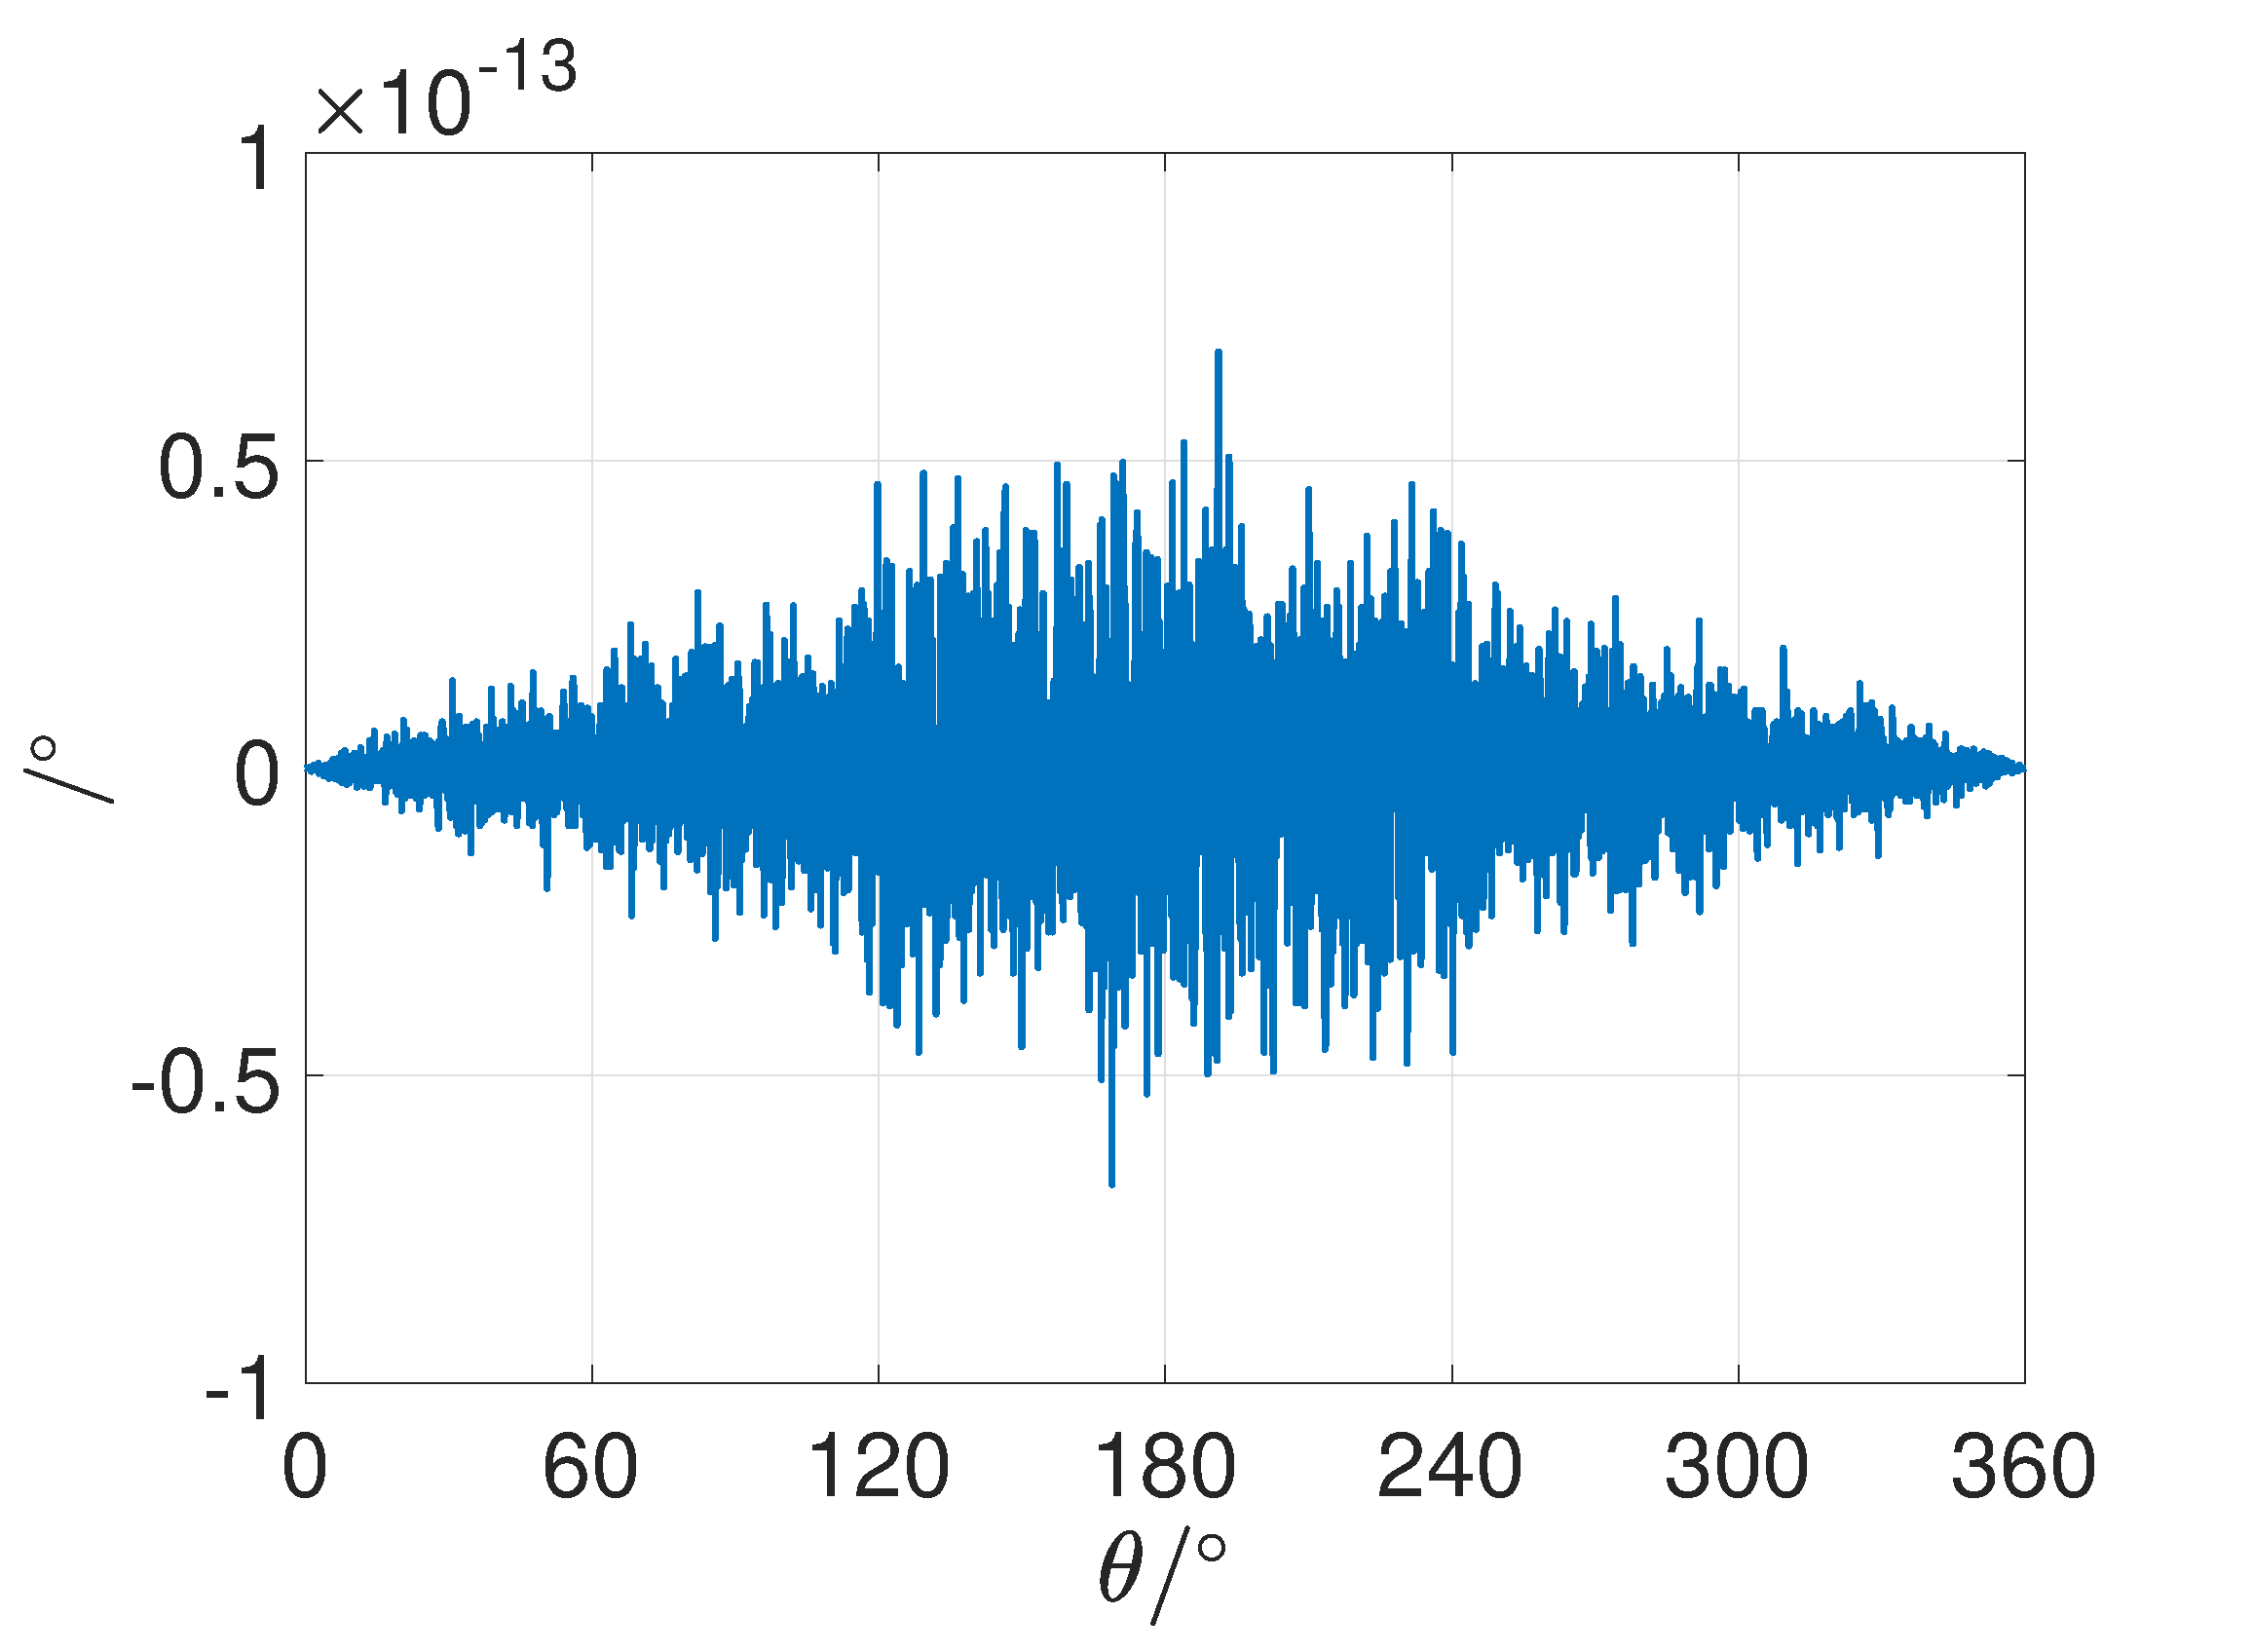
\includegraphics[width=\linewidth]{./Slike/razlika_amp.eps}
		\caption{Razlika med predvideno (\ref{equ:amp_err}) in dejansko napako pri $k=1.1$} \label{fig:razlika}
	\end{center}
\end{figure}




\section{Zaključek}

V članku so predstavljeni poteki napake v odvisnosti od različnih amplitud, enosmernih komponent, faznih zamikov in kombinacije različnih amplitud ter faznih zamikov signalov sinusa in kosinusa. Napaka vsebuje tudi višje harmonike, ki ob večjih razlikah med sinusom in kosinusom niso več zanemarljivi. Za majhna popačenja vhodnih signalov, zadostuje napako izraziti z enosmerno komponento in prvim členom potenčne vrste. Napako izraženo z enosmerno komponento in prvim členom potenčne vrste je potrdila tudi druga literatura \cite{RLS1}. Izraze se lahko uporabi za ugotovitev nepravilne montaže resolverja ali enkoderja, v vgrajenih aplikacijah, kjer ni dostopa do signalov sinus in kosinus. V signalih sinus in kosinus se lahko pojavijo tudi višji harmoniki, ki prav tako vplivajo na napako. Vpliv popačenj vhodnih signalov v  funkcijo atan2 na izhodno napako, ponuja še veliko izzivov za nadaljne delo.


\small
\begin{thebibliography}{1}
\bibitem{uporaba_senzorjev} Gachter J., Hirz M.,Seebacher R., "Impact of Rotor Position Sensor Errors on Speed
Controlled Permanent Magnetized Synchronous
Machines", IEEE 12th International Conference on Power Electronics and Drive Systems (PEDS), pp.822-830, 12-15 Dec. 2017

\bibitem{inkrementalni} Brugnano F., Concari C., Imamovic E., Savi F., Toscani  A., Zanichelli R., "A simple and accurate algorithm for speed measurement in electric drives using incremental encoder",
IECON 2017 - 43rd Annual Conference of the IEEE Industrial Electronics Society, pp. 8551-8556, 29 Oct.-1 Nov. 2017


\bibitem{resolver} Reddy B.P., Murali A., Shaga G., "Low Cost Planar Coil Structure for Inductive Sensors to Measure Absolute Angular
Position", 2017 2nd International Conference on Frontiers of Sensors Technologies (ICFST), pp.14-18, 14-16 April 2017




\bibitem{enkoder} Zhang Z., Ni F., Liu H., Jin M., "Theory analysis of a new absolute position sensor based on electromagnetism", International Conference on Automatic Control and Artificial Intelligence, pp.2204-208, 3-5 Mar. 2012

	
	
\bibitem{RLS1} Qi Lin, T. Li, Z. Zhou, "Error Analysis and Compensation
of the Orthogonal Magnetic Encoder", Proceedings of IEEE ICMCC
Conference, pp.11-14, 21-23 Oct. 2011
\bibitem{RLS2} Hanselman D.C., "Resolver Signal Requirements for High Accuracy
Resolver-to-Digital Conversion", IEEE Transactions on Industrial
Electronics, vol.37, no.6, pp.556-561, Dec. 1990 
\bibitem{RLS3} Demierre M., “Improvements of CMOS Hall Microsystems and
Application for Absolute Angular Position Measurements”, PhD. thesis,
pp. 152-161, Federal Polytechnic School of Lausanne, Switzerland, 2003

\bibitem{mat1} Dolinar G. "Matematika 1", Fakulteta za elektrotehniko, Založba FE in FRI, pp. ,2010

\bibitem{atan} https://www.mathworks.com/help/matlab/ref/atan2.html, dostop junij 2018
\bibitem{atand} https://www.mathworks.com/help/matlab/ref/atan2d.html, dostop junij 2018
\bibitem{fourier} https://sl.wikipedia.org/wiki/Fourierova\_vrsta, dostop junij 2018


\end{thebibliography}

\end{document}
